\chapter{PostScript Stream} \label{Chapter_PostScript}

\section{Introduction}


The {\em PostScript} language is a simple interpretative programming
language with powerful graphics capabilities. Its primary application
is to describe the appearance of text, graphical shapes, and sampled
images on printed pages. A program in this language may be used to
communicate a description of a printable document from a composition
system to a printing system.

 We provide a PostScript output for all geometric
classes which are defined in the \cgal\ kernel.\\
Using this stream allows to create PostScript files which can be viewed,
printed as such or inserted in LaTeX documents.

\begin{ccClass} {PS\_Stream}
\ccSection{The PostScript Stream Class}

\ccDefinition 

An object of type \ccClassName\ is a stream in which geometric
objects and manipulators can be inserted.\\
Every kind of \cgal\ objects introduced into the PostScript stream will
be converted into a PostScript format and put into an output stream
typically linked to a file. The resulting file can be visualized with
a PostScript viewer or sent to any PostScript printer.\\
Such a stream has a state, called {\em context}, that
holds parameters of the drawing such as the current color, or the current line
style \ldots
Contexts can be modified and saved in order to
switch easily between contexts. A \ccClassName\ class also provides
additionnal graphic
features such as a coordinate system, grids, labels and borders.\\
\par
First of all, you have to define a bounding box enclosing all
parts of the objects to be displayed. Objects  
larger than this bounding box, will be clipped. Notice that the
bounding box is given in user's coordinates.\\

Different constants are defined in the \ccClassName\/  class, such as CM, INCH,
POINT.\\
They allow to make a conversion between PostScript dots (1 POINT=1
PostScript dot) and usual units of mesure.\\

Moreover, there exists several modes of output. By default it is the QUIET
mode, which means that the output file will contain no specific information
concerning
the \cgal\ object. It contains only standard  PostScript data, and
therefore can be visualized or printed as such.\\
Alternatively, the QUIET\_EPS mode can be used to create an output which can be
incorporated in a LaTeX document.\\
The READABLE mode inserts in the generated file some PostScript comments
giving a clear description of
each \cgal\ object displayed, that is to say, the position, the
dimensions and the name (point, circle\ldots).\\
And finally, we find the READABLE\_EPS mode, which combines the QUIET\_EPS and
READABLE mode.\\


\ccInclude{CGAL/IO/PS_Stream.h}

\ccTypes
\ccThree{typedef Bbox_2::PS_BBox}{}{bounding box associated to the
output stream}
\ccThreeToTwo

\ccTypedef{typedef const char* DashStyle;}{the style of the dashes.}
\ccGlue 

\ccTypedef{typedef Bbox_2 PS_BBox;}{bounding box associated to the
output stream.}
\ccGlue

\ccNestedType{Context;}{The context type, used to select the drawing
style of the PostScript output.}
\ccGlue

\ccNestedType{Axis;}{The axis type, used to generate a coordinate
system.}
\ccGlue

\ccNestedType{Grid}{The grid type, used to generate a grid.}
\ccGlue

\ccNestedType{Label}{The label type, used to generate labels.}
\ccGlue

\ccNestedType{LaTeX\_Label}{The latex label type, used to generate
LaTeX labels.}
\ccGlue

\ccNestedType{Border}{The border type, used to generate a border
surrounding the bounding box.}
\par
\par  

\ccEnum{enum OutputMode{READABLE, QUIET, READABLE_EPS,
QUIET_EPS};}{The output mode}
\ccEnum{enum DotStyle{NONE, XCROSS, ICROSS, EDOT, FDOT, EBOX,
FBOX};}{The style of points (cf figure~1.1 in section~1.3)}

\ccCreation
\ccCreationVariable{ps}

\ccConstructor{PS_Stream(const PS_BBox& bb, ostream& os,OutputMode
mode=QUIET);}{Creates a PostScript stream associated to the 
bounding box \ccc{bb}, in a \ccc{mode} mode (by default, the mode is
QUIET). The output stream is \ccc{os}. The size of the drawing is
given by a
default value, corresponding to the size of the drawing area on an
A4-paper format.}

\ccConstructor{PS_Stream(const PS_BBox& bb, const char* fname,
OutputMode mode=QUIET);}{Creates the same  PostScript
stream as above, but the output will be a file, named \ccc{fname}.}

\ccConstructor{PS_Stream(const PS_BBox& bb, float H, ostream& os,
OutputMode mode=QUIET);}{This constructor specifies the
size of the drawing in PostScript dots. The \ccc{H}
parameter designs the height of the drawing in PostScript dots. The drawing
width is computed to keep circles round.}

\ccConstructor{PS_Stream(const PS_BBox& bb, float H, const char*
fname, OutputMode mode=QUIET);}{Creates the same
constructor as above, but the output stream will be in a file, named
\ccc{fname}.}

\ccConstructor{PS_Stream(const PS_BBox& bb, float L, float H, ostream& 
os, OutputMode mode=QUIET);}{This constructor specifies the 
size of the PostScript drawing, in PostScript dots. The \ccc{L}
parameter represents the width of the output, and \ccc{H} the height.}

\ccConstructor{PS_Stream(const PS_BBox& bb,float L, float H, const
char* fname, OutputMode mode=QUIET);}{Creates the same
constructor as above, but the output stream will be in a file, named
\ccc{fname}.}

\ccThree{const Context&&}{}{Creates the same constructor as above, but th}

\ccFunction{void ~PS_Stream();}{The destructor. Inserts all the LaTeX
instructions (if any), all the LaTeX labels (if any) and closes the stream.}


\ccAccessFunctions
\par

\ccMethod{ostream& os();}{Returns the stream in which goes the
PostScript output.}
\ccGlue

\ccMethod{List_Label& list();}{Returns the list of LaTeX labels.}
\ccGlue

\ccMethod{const Context context() const;}{Returns the context.}
\ccGlue

\ccMethod{PS_BBox bbox() const;}{Returns the bounding box associated
to the PostScript stream.}
\ccGlue

\ccMethod{int width() const;}{Returns the width of the output.}
\ccGlue

\ccMethod{int height() const;}{Returns the height of the output.}
\ccGlue

\ccMethod{OutputMode mode();}{Returns the output Mode.}
\ccGlue

\ccMethod{double xratio();}{Returns the scale for the x-axis.}
\ccGlue

\ccMethod{double yratio();}{Returns the scale for the y-axis.}
\ccGlue

\ccMethod{bool is_eps();}{Returns \ccc{true} if the output mode is
QUIET\_EPS or READABLE\_EPS.}
\ccGlue

\ccMethod{bool is_readable();}{Returns \ccc{true} if the output mode 
is READABLE or READABLE\_EPS.}
\ccGlue

\ccOperations

\ccFunction{double x2ps(double x);}{Converts user's coordinates in  PostScript's coordinates.}
\ccGlue

\ccFunction{double y2ps(double y);}{Converts user's coordinates in PostScript's coordinates.}
\par
\par

\ccHeading{Setting functions}

The following member functions allow to change the state of the stream, by
modifying the data members of the \ccc{Context}\ class. They allow
to change the color, the line width, the line style\ldots. \\
The same effects are more typically achieved by \ccc{manipulators} inserted
in the PostScript stream. These \ccc{manipulators} are described in section ~1.4.
\par


\ccFunction{PS_Stream& set_border_color(const Color& c);}{Allows to
change the color of border lines.}
\ccGlue

\ccFunction{PS_Stream& set_fill_color(const Color& c);}{Allows to fill
closed figures in a chosen color.}
\ccGlue

\ccFunction{PS_Stream& set_point_size(unsigned int s);}{Allows to change
the point size.}
\ccGlue

\ccFunction{PS_Stream& set_line_width(unsigned int t);}{Allows to change
the line thickness.}
\ccGlue

\ccFunction{PS_Stream& set_point_style(DotStyle style);}{Allows to
change the point style.}
\ccGlue

\ccFunction{PS_Stream& set_line_style(DashStyle style);}{Allows to change the 
line style.}
\ccGlue

\ccFunction{PS_Stream& set_fill(bool b);}{To fill or not a closed
figure. If \ccc{true} the figure is filled.}
\ccGlue

\ccFunction{PS_Stream& set_default_context(void );}{Allows to come back
to the default context.}
\ccGlue

\ccFunction{PS_Stream7 set_current_contex(const Context& c);}{Allows
to globally change the context into an other.}
\ccGlue

\ccFunction{PS_Stream& set_point(Point_2<Cartesian<double>> p);}{Allows to 
change the position of the anchor point.}
\ccGlue

\ccFunction{PS_Stream& set_axis(Axis& a);}{Used to generate a
coordinate system.}
\ccGlue

\ccFunction{PS_Stream& set_grid(Grid& g);}{Used to generate a Grid.}
\ccGlue

\ccFunction{PS_Stream& put_ps_label(const char* txt);}{Used to create a
standard label.}
\ccGlue

\ccFunction{PS_Stream& put_latex_label(const char* txt);}{Used to create a
LaTeX label.}
\ccGlue

\ccFunction{PS_Stream& put_border(unsigned int t);}{Used to generate a 
frame around the drawing.}
\ccGlue

\ccFunction{PS_Stream& set_font(const char* ch);}{Allows to change the
name of the font, for standard labels.}
\ccGlue

\ccFunction{PS_Stream& set_font_size(unsigned int s);}{Allows to change
the size of the font, for standard labels.}
\par


As you saw in the \ccc{PS\_Stream} class, we had to introduce some 
auxiliary classes which define the graphical environment. These
following classes are members of the \ccClassName\ class.

\end{ccClass}

\section{Included classes of the PS\_Stream class}

\begin{ccClass} {Context}
\ccSubsection{Context class}

\ccDefinition

An object of the \ccClassName\ class defines a graphical context. It is used 
to select the drawing style of points, lines, the colors \ldots.
\ccClassName\ is a member class of the PS\_Stream class.\\

The current context can be modified by using
different functions that allow to directly change the parameters of the
\ccClassName\ class or by
inserting manipulators in the PostScript stream (cf section ~1.4 {\em manipulators}).\\ 

There is a default \ccClassName. \\
The default values of the different fields of this class are : \\
\\
\par
\begin{tabbing}
Border color border color \= \kill
Border Color     \>            BLACK\\
Fill Color       \>            BLACK\\
Fill             \>            FALSE\\
Dot Style        \>            XCROSS\\
Dot Size         \>            5\\
Thickness        \>            0\\
Line Style       \>            SOLID\\
Font Size        \>            12\\
Font             \>            ``Helvetica''\\
Anchor Point     \>            (0,0)\\
\end{tabbing}

The following figure shows the different kinds of style of points and lines.

\begin{figure}[h]
\includegraphics{PS_Stream/style.ps}
\caption{DOT STYLE AND DASH STYLE}
\end{figure}

\ccCreation
\ccCreationVariable{c}

\ccConstructor{PS_Stream::Context();}{Creates a default context.}

\ccConstructor{PS_Stream::Context(const Context&
ctxt);}{Copy constructor.}

\ccAccessFunctions

\ccMethod{Color get_border_color() const;}{Returns the border color.}
\ccGlue

\ccMethod{Color get_fill_color() const;}{Returns the color used to
fill and draw the figures.}
\ccGlue

\ccMethod{DotStyle get_dot_style() const;}{Returns the dot style (cf figure ~1.1).}
\ccGlue

\ccMethod{unsigned int get_dot_size() const;}{Returns the dots size
(given in PostScript dots).}
\ccGlue

\ccMethod{unsigned int get_thickness() const;}{Returns the lines
thickness (given in PostScript dots).}
\ccGlue

\ccMethod{unsigned int get_font_size() const;}{Returns the font size,
used only for standard labels.}
\ccGlue

\ccMethod{DashStyle get_line_style() const;}{Returns the line style (cf 
 figure ~1.1).}
\ccGlue

\ccMethod{const char* get_font() const;}{Returns the name of the
font, used only for standard labels.}
\ccGlue

\ccMethod{bool get_fill() const;}{Returns true if a polygon is filled.}
\par



\ccMethod{Point_2<Cartesian <double>> get_pos() const;}{Returns the
position of the anchor point.}
\ccGlue


\ccOperations

\ccMethod{void set_border_color(const Color& c);}{Sets the border
color.}
\ccGlue

\ccMethod{void set_fill_color(const Color& c);}{Sets the fill color.}
\ccGlue

\ccMethod{void set_dot_style(DotStyle& s);}{Sets the dot style.}
\ccGlue

\ccMethod{void set_dot_size(unsigned int s);}{Sets the dot size given
in PostScript dots.}
\ccGlue

\ccMethod{void set_thickness(unsigned int t);}{Sets the line
thickness given in PostScript dots.}
\ccGlue

\ccMethod{void set_font_size(unsigned int s);}{Sets the font size.}
\ccGlue

\ccMethod{void set_fill(bool& b);}{Closed figures will be filled if
\ccc{b=true}.}
\par

\ccMethod{void set_current_pos(const Point_2<Cartesian <double>>&
p);}{Point p becomes the current position.}
\ccGlue

\ccMethod{void set_line_style(DashStyle style);}{Sets the line style
to \ccc{style}.}
\ccGlue

\ccMethod{void set_font(const char* font);}{Sets the font. You must
use the PostScript names of font.}
\par

The selected font and font size apply only to the standard labels. The font
and font size of LaTeX labels are of the responsability of the LaTeX
environment.

\end{ccClass}

\begin{ccClass}{Axis}
\ccSubsection{Axis class}

\ccDefinition
An object of the \ccClassName\ class allows you to represent axis on the
PostScript output, therefore a coordinate system.
An object of such a class is defined by two doubles and one
integer.
The two doubles define the step between two marks on the x-axis 
and the y-axis (a zero value means no mark displayed on the axis).
The integer represents the thickness of the axis.
Only one \ccClassName\ object can be inserted in a PostScript stream.

\ccCreation
\ccCreationVariable{a}

\ccConstructor{PS_Stream::Axis();}{Creates an orthonormal coordinate
system, with a line thickness 0.}

\ccConstructor{PS_Stream::Axis(double x,double y,unsigned int
t=0);}{Creates an orthogonal coordinate system with steps \ccc{x} and
\ccc{y} and the line thickness \ccc{t} (by default \ccc{t=0}).}

\ccConstructor{PS_Stream::Axis(double xy,unsigned int t=0);}{Creates
an orthogonal coordinate system with the same step \ccc{xy} for x-axis
and y-axis and the line thickness t (by default t=0).}

\ccAccessFunctions

\ccMethod{double stepx() const;}{Returns the step of the x-axis.}
\ccGlue

\ccMethod{double stepy() const;}{Returns the step of the y-axis.}
\ccGlue

\ccMethod{unsigned int thickness() const;}{Returns the thickness of the
axis.}
\par


\end{ccClass}

\begin{ccClass}{Grid}
\ccSubsection{Grid class}

\ccDefinition
An object of the \ccClassName\ class allows you to represent a grid on the 
output stream, that is to say, sequences of parallel lines equally
spaced.
An object of such a class is defined by two doubles and a DashStyle.
The two doubles represent the vertical and horizontal spacing, and the 
DashStyle the style of lines (cf figure ~1.1).
Contrary to the objects of type \ccc{Axis}, you can insert as many
\ccClassName\ object as you want in a PostScript stream.

\ccCreation
\ccCreationVariable{g}

\ccConstructor{PS_Stream::Grid();}{Creates a grid with lines spaced of 
1.0 and a default dash style (''[1 5] 0''). The style is the dash style used by PostScript.}

\ccConstructor{PS_Stream::Grid(double x, double y, DashStyle str=''[1
5] 0'');}{Creates a grid with vertical lines spaced of \ccc{x},
horizontal lines spaced of \ccc{y} and dash style \ccc{str}.}

\ccConstructor{PS_Stream::Grid(double xy, DashStyle str=''[1 5]
0'');}{Creates a grid with the same lines spacing \ccc{xy} and dash style \ccc{str}.}

\ccAccessFunctions

\ccMethod{double stepx() const;}{Returns the spacing between the
vertical lines.}
\ccGlue

\ccMethod{double stepy() const;}{Returns the spacing between the
horizontal lines.}
\ccGlue

\ccMethod{DashStyle style() const;}{Returns the line style.}
\par


\end{ccClass}

\begin{ccClass}{Label}
\ccSubsection{Label class}

\ccDefinition
This class is used to insert text in a PostScript output.
An object of the \ccClassName\ class is a label, that is to say text that can be inserted in a PostScript stream.
The text will be displayed at the anchor point with the font and the
font size of the current context.

\ccCreation
\ccCreationVariable{l}

\ccConstructor{PS_Stream::Label();}{Creates an empty label, with no
text.}

\ccConstructor{PS_Stream::Label(const char* txt);}{Creates a label
with \ccc{txt} as text.}

\ccAccessFunctions

\ccMethod{char* text() const;}{Returns the label text.}
\par

\end{ccClass}

\begin{ccClass}{LaTeX_Label}
\ccSubsection{LaTeX\_Label class}

\ccDefinition
This class is used to insert labels in drawing that are to be inserted 
in a LaTeX document.
Such labels will appear with the font and font size of the including
LaTeX document.
However, you can
change this parameters by using standard LaTeX commands within the labels.\\
The PostScript stream must be created with the mode QUIET\_EPS or READABLE\_EPS.\\
These labels won't be display with a viewer but only with LaTeX, by
the following way :
the generated PostScript file, for example \ccc{drawing.ps}, is then
included in a LaTeX document as an {\sc Ipe} file by using the
following syntax :

\begin{verbatim}
\documentclass[]{article}
\begin{document}
\def\Ipe#1{\def\IPEfile{#1}\input{#1}}
...
\Ipe{drawing.ps}
...
\end{document}
\end{verbatim}


\ccCreation
\ccCreationVariable{l}

\ccConstructor{PS_Stream::LaTeX_Label();}{Creates a LaTeX label with
no text.}

\ccConstructor{PS_Stream::LaTeX_Label(const char* txt);}{Creates a
LaTeX label with \ccc{txt} as text.}

\end{ccClass}

\begin{ccClass}{Border}
\ccSubsection{Border class}

\ccDefinition
The \ccClassName\ class is used to insert a frame surrounding the bounding box
into the stream.

\ccCreation
\ccCreationVariable{b}

\ccConstructor{PS_Stream::Border(int s =0);}{Creates a border of
thickness \ccc{s} (by default \ccc{s=0}).}

\ccAccessFunctions

\ccMethod{int size() const ;}{Returns the border thickness.}
\ccGlue

\end{ccClass}
\par


\section{Manipulators}

A \ccc{manipulator} is an object which can be inserted in a PostScript 
stream, via the operator <<, to change the context for further
drawing.\\
The \ccc{manipulators} are inserted in the PostScript stream through
 \ccc{manipulator-creators}, a \ccc{manipulator-creator} being  an 
object function whose operator () creates a \ccc{manipulator}.\\
Thus, to change the state of a stream, users just need to insert in
the stream a \ccc{manipulator} created by the operator () of a
\ccc{manipulator-creator} writing for exemple : \\
 ps << line\_width(4) << segment; to change the width of a segment.\\

Here, we simply document the use of these operators which is all the
user needs to know  to modify the state of a stream. The design of
\ccc{manipulators} and \ccc{manipulator-creator} being given after.\\

\ccThree{PS_Stream&}{PS_Stream& ps << current\_context()}{}

\ccFunction{PS_Stream& operator<<(PS_Stream& ps,border\_color(const
Color& c));}{Sets the color used to draw objects.}
\ccGlue

\ccFunction{PS_Stream& operator<<(PS_Stream& ps,fill\_color(const
color& c));}{Sets the color used to fill objects.}
\ccGlue

\ccFunction{PS_Stream& operator<<(PS_Stream& ps,point\_size(unsigned
int s));}{Sets the point size in PostScript dots.}
\ccGlue

\ccFunction{PS_Stream& operator<<(PS_Stream& ps, point\_style(enum
DotStyle style));}{Modify the representation of points.}
\ccGlue

\ccFunction{PS_Stream& operator<<(PS_Stream& ps, line_style(DashStyle
style));}{Modify style of lines.}
\ccGlue

\ccFunction{PS_Stream& operator<<(PS_Stream& ps, line_width(unsigned
int t));}{Sets the line thickness in PostScript dots.}
\ccGlue

\ccFunction{PS_Stream& operator<<(PS_Stream& ps, fill(bool b));}{Sets
if closed figures must be filled (\ccc{true})\/ or not
(\ccc{false})\ .}
\ccGlue

\ccFunction{PS_Stream& operator<<(PS_Stream& ps, current_context(const
Context& c));}{Changes the context.}
\ccGlue


\ccFunction{PS_Stream& operator<<(PS_Stream& ps,
move_to(Point_2<Cartesian<double>> p));}{Sets the current anchor
point.}
\ccGlue

\ccFunction{PS_Stream& operator<<(PS_Stream& ps, show_axis(Axis&
a));}{Draws axis.}
\ccGlue

\ccFunction{PS_Stream& operator<<(PS_Stream& ps, show_grid(Grid&
g));}{Draws a grid.}
\ccGlue

\ccFunction{PS_Stream& operator<<(PS_Stream& ps, ps_label(const char*
txt));}{Puts a standard label at the anchor point.}
\ccGlue

\ccFunction{PS_Stream& operator<<(PS_Stream& ps, latex_label(const
char* txt));}{Puts a LaTeX label at the anchor point.}
\ccGlue

\ccFunction{PS_Stream& operator<<(PS_Stream& ps, border(unsigned
int t));}{Draws borders surrounding the bounding box.}
\ccGlue

\ccFunction{PS_Stream& operator<<(PS_Stream& ps, font(const char*
ch));}{Sets the font of the PostScript label output, only for
standard labels.}
\ccGlue

\ccFunction{PS_Stream& operator<<(PS_Stream& ps, font_size(unsigned
int s));}{Sets the font size of PostScript label output, only for standard
labels.}
\par

\begin{ccAdvanced}

The next paragraph makes precise, for the advanced users, the design of
\ccc{manipulators} and \ccc{manipulator-creators}.


\begin{ccClassTemplate}{PS_Manipulator<T>}
\ccSubsection{PS\_Manipulator class}

A \ccClassTemplateName\ is an object which can be inserted in a
PostScript stream to modify the context of this stream.

An object of the \ccClassTemplateName\ class is created with a pointer
to a function f and an object of type \ccc{T}. This 
function is a setting member of the \ccc{PS_Stream} class, it has only one
argument of type \ccc{T} and returns a \ccc{PS_Stream} object. Notice
that \ccc{T} is the type of the \ccc{Manipulator} argument.

\ccCreation
\ccCreationVariable{psm}

\ccConstructor{PS_Manipulator<T>(PS_Stream& (PS_Stream::*f)(T), T
t);}{}

\end{ccClassTemplate}

To change the state of the stream, a \ccc{PS_Manipulator} can be
inserted in the PostScript stream via the output operator <<, defined as follow :

\ccHeading{I/O}

 
\ccGlobalFunction{PS_Stream& operator<<(PS_Stream& pss, const PS_Manipulator<T>
& psm);}{Triggers a call to \ccc{pss.f(t)}.}

\begin{ccClassTemplate}{PS_Manipulator_creator<T>}
\ccSubsection{PS\_Manipulator\_creator class}

A \ccClassTemplateName\ is an object function whose operator ()
produces the creation of a \ccc{manipulator}.\\
This class is templated by a type \ccc{T} and its creator takes as
argument the pointer to a setting function, member of the
\ccc{PS\_Stream} class, with an argument of type \ccc{T}.

\ccCreation
\ccCreationVariable{psmc}

\ccThree{PS_Manipulator_creator<T>}{}{Allows to obtain from a function of 
type}
\ccThreeToTwo

\ccConstructor{PS_Manipulator_creator(PS_Stream& (PS_Stream::* f)(T))}{}

\ccMethod{PS_Manipulator<T> operator()(T param);}{Returns a
PS\_Manipulator object whose operator << triggers the call to f(T).}



\end{ccClassTemplate}

\subsection{The PS\_Manipulator\_creator}

\cgal\ offers for the \ccc{PS\_Stream} class, the following
\ccc{manipulators-creators} :


\def\ccLongParamLayout{\ccFalse}

\ccFunction{PS_Manipulator_creator<const Color&>
border_color(&PS_Stream::set_border_color);}{Sets the color used to 
draw the boundaries objects.}
\ccGlue

\ccFunction{PS_Manipulator_creator<const
Color&> fill_color(&PS_Stream::set_fill_color);}{Sets the color used 
to fill objects.}
\ccGlue

\ccFunction{PS_Manipulator_creator<unsigned int>
point_size(&PS_Stream::set_point_size);}{Sets the points size in
PostScript dots.}
\ccGlue

\ccFunction{PS_Manipulator_creator<PS_Stream::DotStyle>
point_style(&PS_Stream::set_point_style);}{Modifies the
representation of points.}
\ccGlue

\ccFunction{PS_Manipulator_creator<DashStyle>
line_style(&PS_Stream::set_line_style);} {Modifies the style of lines.}
\ccGlue

\ccFunction{PS_Manipulator_creator<unsigned int>
line_width(&PS_Stream::set_line_width);} {Sets the line thickness in
PostScript dots.}
\ccGlue

\ccFunction{PS_Manipulator_creator<bool>
fill(&PS_Stream::set_fill);} {Sets if closed figures must be
filled (\ccc{true})\  or not (\ccc{false})\ .}
\ccGlue

\ccFunction{PS_Manipulator_creator<const PS_Stream::Context&>
current_context(&PS_Stream::set_current_context);}{Changes the context.}
\ccGlue


\ccFunction{PS_Manipulator_creator<Point_2<Cartesian<double>>>
move_to(&PS_Stream::set_point);}{Sets the current anchor point.}
\ccGlue
\par 

\ccFunction{PS_Manipulator_creator<PS_Stream::Axis&>
show_axis(&PS_Stream::set_axis);}{Draws axis.}
\ccGlue
\par

\ccFunction{PS_Manipulator_creator<PS_Stream::Grid&>
show_grid(&PS_Stream::set_grid);}{Draws a grid.}
\ccGlue
\par

\ccFunction{PS_Manipulator_creator<const char*>
ps_label(&PS_Stream::put_ps_label);}{Puts a standard label at the
anchor point.}
\ccGlue

\ccFunction{PS_Manipulator_creator<const char*>
latex_label(&PS_Stream::put_latex_label);}{Puts a LaTeX label at
the anchor point.}
\ccGlue

\ccFunction{PS_Manipulator_creator<unsigned int>
border(&PS_Stream::put_border);}{Draws borders.}
\ccGlue
\par

\ccFunction{PS_Manipulator_creator<cont char*>
font(&PS_Stream::set_font);}{Sets the font of the PostScript label 
output, only for standard labels.}
\ccGlue

\ccFunction{PS_Manipulator_creator<const char*>
font_size(&PS_Stream::set_font_size);}{Sets the font size of PostScript
label output, only for standard labels.}
\ccGlue

\end{ccAdvanced}

\ccHeading{I/O}

Each geometric class of \cgal\ gets its own output operator for the
PostScript stream provided by \cgal.

\ccInclude{CGAL/IO/PostScript_stream.h}

\ccThree{PS_Stream& ps}{PS_Stream& ps << X}{}

\ccFunction{PS_Stream& operator<<(PS_Stream& ps, const
PS_Stream::Border& b);}{Inserts the border \ccc{b} into the stream
\ccc{ps}, surrounding the bounding box.}
\ccGlue

\ccFunction{PS_Stream& operator<<(PS_Stream& ps, const
PS_Stream::Label& txt);}{Displays the label \ccc{txt} at the anchor
point.}
\ccGlue

\ccFunction{PS_Stream& operator<<(PS_Stream& ps, const
PS_Stream::LaTeX_label& txt);}{Displays the LaTeX label \ccc{txt} at
the anchor point, \ccc{only in a LaTeX document}.}
\ccGlue

\ccFunction{PS_Stream& operator<<(PS_Stream& ps, const
PS_Stream::Grid& g);}{Inserts the grid \ccc{g} into the stream
\ccc{ps}.}
\ccGlue

\ccFunction{PS_Stream& operator<<(PS_Stream& ps, const
PS_Stream::Axis& a);}{Inserts the coordinate system \ccc{a} into the
stream \ccc{ps}.}
\ccGlue

\ccFunction{PS_Stream& operator<<(PS_Stream& ps, const Point_2<R>&
p);}{Inserts the point \ccc{p} into the stream \ccc{ps}.}
\ccGlue

\ccFunction{PS_Stream& operator<<(PS_Stream& ps, const Segment_2<R>&
s);}
{Inserts the segment \ccc{s} into the stream \ccc{ps}.}
\ccGlue

\ccFunction{PS_Stream& operator<<(PS_Stream& ps, const Line_2<R>&
l);}{Inserts the line \ccc{l} into the stream \ccc{ps}.}
\ccGlue

\ccFunction{PS_Stream& operator<<(PS_Stream& ps, const Ray_2<R>&
r);}{Inserts the ray \ccc{r} into the stream \ccc{ps}.}
\ccGlue

\ccFunction{PS_Stream& operator<<(PS_Stream& ps, const Parabola<R>&
p);}{Inserts the parabola \ccc{p} into the stream \ccc{ps}.}
\ccGlue

\ccFunction{PS_Stream& operator<<(PS_Stream& ps, const Triangle_2<R>&
t);}{Inserts the triangle \ccc{t} into the stream \ccc{ps}.}
\ccGlue

\ccFunction{PS_Stream& operator<<(PS_Stream& ps, const
Iso_rectangle_2<R>& r);}{Inserts the iso rectangle \ccc{r} into the
stream \ccc{ps}.}
\ccGlue

\ccFunction{PS_Stream& operator<<(PS_Stream& ps, const Circle_2<R>&
c);}{Inserts the circle \ccc{c} into the stream \ccc{ps}.}
\ccGlue

\ccExample

The following code fragment would allow you to have a look of the
main functions associated to the PostScript output, and their usage.

\begin{cprog}

#include <iostream>
#include <fstream>

#include <CGAL/Cartesian.h>
#include <CGAL/Point_2.h>
#include <CGAL/Segment_2.h>
#include <CGAL/Triangle_2.h>
#include <CGAL/Iso_rectangle_2.h>
#include <CGAL/Ray_2.h>
#include <CGAL/Circle_2.h>
#include <CGAL/IO/PS_Stream.h>

typedef CGAL::Point_2< CGAL::Cartesian<double> >     Point;
typedef CGAL::Segment_2< CGAL::Cartesian<double> >   Segment;
typedef CGAL::Ray_2< CGAL::Cartesian<double> >       Ray;
typedef CGAL::Triangle_2< CGAL::Cartesian<double> >  Triangle;
typedef CGAL::Iso_rectangle_2< CGAL::Cartesian<double> > Rect;
typedef CGAL::Circle_2< CGAL::Cartesian<double> >    Circle;
typedef CGAL::Bbox_2 BBox;

int  main()
{

CGAL::PS_Stream::PS_BBox bb(-2,-2,2,2);
CGAL::PS_Stream ps(bb,300,"toto.ps",CGAL::PS_Stream::QUIET_EPS);

CGAL::PS_Stream::Grid g(0.5,0.5);
CGAL::PS_Stream::Axis a(1.0,1.0);
Point p(-1,1), q(1,1), r(1,-1), s(-1,-1),som(0,2), b1(-0.5,1.5),
   b2(0.5,1.5), o(0,0);

Triangle tr(b1,b2,som);
Circle ci(o,1.0);
CGAL::PS_Stream::Label l1("Centre");

ps << p;
ps << CGAL::line_width(2);    
ps << point_style(CGAL::PS_Stream::FDOT) << q;
ps << point_style(CGAL::PS_Stream::FBOX) << r;
ps << point_style(CGAL::PS_Stream::ICROSS) << s;
 ps << CGAL::fill(true) <<
fill_color(CGAL::Color(0,255,0))<<border_color(CGAL::Color(0,0,255))<<ci;
ps << move_to(Point(0.15,0.1)) << CGAL::font("Helvetica-Oblique")<< l1;
ps << CGAL::fill(false)<<border_color(CGAL::Color(255,0,255))<< tr;
ps << current_context(CGAL::CTXT_DEFAULT);
ps << move_to(Point(0.6,1.5)) <<CGAL::ps_label("triangle");
ps <<a;
ps <<show_grid(g);
ps <<CGAL::border(3);

return 0;
}


\end{cprog}

and after visualisation, you obtain :\\
\\

\begin{figure}[h]
\begin{center}
\includegraphics{PS_Stream/exemple.ps}
\end{center}
\caption{PostScript output}
\end{figure}


